%
%\section{ГЛАВА 1.}
%\subsection{1.1. Последовательность определения стоимости Объекта}
%
%

\section{Описание объекта исследования}

Исследуемая дизельная электростанция используется для обеспечения резервного питания медицинского учреждения, когда  отключение главных и вспомогательных потребителей может привести к аварии или человеческим жертвам

\par Из предоставленных материалов   специалистом  установлена следующая общая информация об объекте исследования, имеющая значение для дачи заключения:
\parbox[90mm]{10cm}{}
\begin{itemize}
	\item[ ] 
	\begin{description}
		\item[Марка, модель] \hfill South Power АД 30 - Т400
		%		\item[Обозначение модели] \hfill \model  
		\item[Номинальная мощность] \hfill 32 кВт
		\item[Количество фаз] \hfill 3
    	\item[Напряжение] \hfill 400/230 В
	%	\item[Год выпуска] \hfill \год
		\item[Номер шасси] \hfill отсутствует
		\item[Цвет ЛКП] \hfill красный
		\item[Наработка] \hfill  296  моточасов
		%	\item[Дата начала эксплуатации] \hfill \началоэкспл
		\item[Год производства] \hfill 2013 
		\item[Двигатель] \hfill YangDong Y4102D
		\item[Генератор] \hfill Azimut Z184H1
		%	\item[Объем двигателя] \hfill 1328 $ \text{см}^3 $
	%	\item[Свидетельство о регистрации] \hfill \свид
		%	\item[ПТСШ
		\item[Масса] \hfill 1020 кг
	\item[Страна изготовитель] \hfill Россия
	\end{description}
\end{itemize}

\subsection{ Характеристика объекта }
\subsubsection{Дизельная электростанция South Power AD 30 - T400}


\дварядом{1}{South Power AD 30 - T400. Вид спереди слева}{2}{South Power AD 30 - T400. Вид сзади слева}

\begin{figure}[H]
	\centering
	\includegraphics[width=0.99\linewidth]{example-image}
	\caption[]{Маркировочная табличка объекта исследования дизельная электростанция South Power AD 30 - T400}
\end{figure}

\begin{figure}[H]
	\centering
	\includegraphics[width=0.99\linewidth]{example-image}
	\caption{Инвентарный номер исследуемого объекта}
	\label{fig:инв}
\end{figure}



\subparagraph{Краткая характеристика основных узлов исследуемого объекта}

\subparagraph{Привод силовой дизельный - PDYn-60(Y4102D)} автономная силовая единица, состоящая из двигателя с глушителем и радиатора, установленных на едином подрамнике, на виброопорах. Привод предназначен для резервной или автономной работы в составе агрегатов коммунальных машин, строительной и сельскохозяйственной техники, в пожарных, бытовых, нефте и дизель перекачивающих насосах, оросительной технике, промышленных шредерах, дробилках, лебедках, гидростанциях и многом другом. Дизельный привод RD4102 - состоит из рядного, 4-х тактного, дизельного двигателя, жидкостного охлаждения производства компании YangDong. Мощность составляет 63кВт / 85лс при 3000 об.мин. Максимальный крутящий момент 99.8Нм. Дизельный привод RD4102, может быть укомплектован пультом(панелью/шкафом) управления с требуемым функционалом.

\дварядом{example-image}{Привод силовой дизельный - PDYn-60}{example-image}{Габаритные размеры привода PDYn-60}
%
%
\subparagraph{Четырёхцилиндровый рядный дизельный двигатель} объемом 3.87 л. жидкостного охлаждения китайского производства максимальной мощностью 36.3 кВт (49.4 л.с.) с частотой вращения 1500 оборотов в минуту предназначен для использования на энергетических силовых установках или аналогичном промышленном оборудовании.  Унифицированные габаритны, посадочные и присоединительные размеры двигателя Y4102D допускают установку вместо дизельных двигателей Kubota, Yanmar, Lombardini, KIPOR, ММЗ, ЯМЗ.

\begin{figure}[H]
	\centering
	\includegraphics[width=0.99\linewidth]{example-image}
	\caption{Основные характеристики двигателя Y4102D}
	\label{fig:12}
\end{figure}

\begin{figure}[H]
	\centering
	\includegraphics[width=0.9\linewidth]{example-image}
	\caption[]{Диаграмма мощности и крутящего момента двигателя PDYn-60}
\end{figure}


\subparagraph{Генератор  
	Azimut} модели  Z184HI с контроллером   
	Smartgen HGM 6120U.
	
	Основные характеристики генератора представлены ниже в таблице на рис. \ref{fig:123}:\\
		
\begin{figure}[H]
	\centering
	\includegraphics[width=0.99\linewidth]{example-image}
	\caption{Технические характеристики генератора Z1884HI}
	\label{fig:123}
\end{figure}

	
	
%	
%	\begin{figure}[H]
%		\centering
%		\includegraphics[width=0,8\linewidth]{images/jpg/гнр}
%		\caption{Краткие технические характеристики генератора Azimut} модели Z184HI}
%	\label{fig:2}
%\end{figure}
%
\subparagraph {Контроллер автозапуска генератора} Smartgen HGM6120U принадлежит серии HGM6100U и используется для автоматического управления генератором. Выполняет функцию автоматического пуска/останова, измерение данных и три функции удаленного управления. Все необходимые параметры настраиваются на передней панели контроллера или посредством программирования через компьютер (через USB-порт). 
	
	\дварядом{example-image}{Панель управления Smartgen HGM 6120U}{example-image}{Панель управления Smartgen HGM 6120U}


\subsection{Текущее использование объекта исследования}

Исследуемая \тс \ находится в неработоспособном состоянии и непригодня для использования по своему прямому назначению.

%\begin{figure}[H]
%	\centering
%	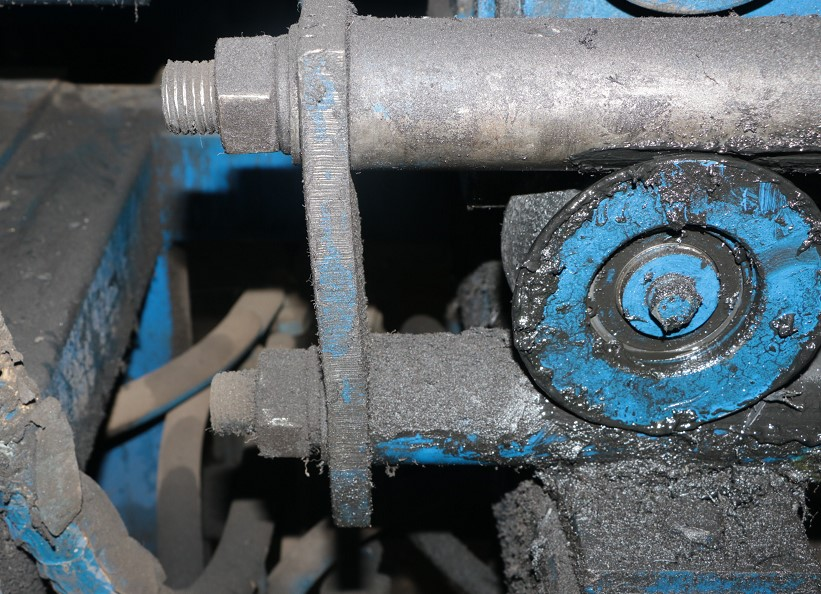
\includegraphics[width=0.9\linewidth]{images/jpg/10}
%	\caption{\tc. Вид на двигатель слева в момент пробного запуска}
%	\label{fig:10}
%\end{figure}

\subsubsection{История ремонта и сервисного обслуживания}

Исследование истории и сервисного обслуживания дизельного генератора специалистом не производилось ввиду непредоставления специалисту надлежащих документов.



\subsection{Исследование физического состояния }

\subsubsection{Осмотр дизельного генератора}

\osm\, специалистом проведёно исследование  	дизельной электростанции South Power AD 30 - T400  № 201310202 2013 года выпуска, инв. № 42910001017. Исследование  проводилось в сухую, ясную погоду с 12-00  до 18-00 на открытой площадке   по адресу: \местоосмотра.   На начало осмотра двери металлического корпуса генератора открыты.  Соответствие марки, модели,  номера  исследуемого генератора записям в договоре на производство исследования и предоставленной инвентарной карточке учета соответствует.


Внешним осмотром генератора установлено следующее: снаружи корпус  электрогенераторной установки и  двигателя внутреннего  сгорания окрашены эмалью красного цвета. Блок двигателя и частично навесное оборудование забрызганы жидкостью, содержащей   вещество темного цвета.     Уровень масла в ДВС значительно больше нормы, выше верхней отметки щупа, масло темное, прозрачное, с запахом моторного топлива.  Уровень охлаждающей жидкости в норме.  

Видимые, внешние признаки повреждения электро-генераторной установки отстутствуют, за исключением незначительного изменения тона окраски блока цилиндров дизельного двигателя в задней части.

Видимые, внешние признаки повреждений системы охлаждения двигателя отсутствуют.

Электронная система дизельного генератора без видимых повреждений.

%Система запуска двигателя исправна.

Запуск двигателя без электрической нагрузки показал наличие  значительной неисправности ДВС.  В начальный период работа двигателя нестабильна, сопрождается нефункциональными шумами, значительным задымлением. Выхлоп густой, сизе-синий. 

Ввиду явной неисправности двигателя диагностирование и исследование электростанции в рабочем режиме было остановлено. 


С целью установления причины и степени повреждения ДВС в процессе осмотра было принято совместное решение с представителем заказчика о разборке дизельного двигателя.


Демонтаж и разбрка ДВС, а так же  другие сопутствующие работы, необходимые для проведения экспертного исследования, выполнялись персоналом заказчика  в соответствии с заданиями специалиста.  

Слитая жидкость из системы охлаждения темно-оранж цвета, с включениями мелкодисперсных твердых частиц. Размер частиц не превышает 0,2-0,3 мм. Возможные признаки загрязнеия жидкости  системы охлаждения  моторным топливом или моторным маслом отсутствуют.  

После слива моторного масла из блока ДВС на дне картера видны множественные   металлические  магнитные и не магнитные  частицы. На сетке маслозаборника присутсвует небольшое количество крупных металлических частиц и частиц вещества темного цвета. Вязкость моторного масла низкая, моторное масло с характерным запахом дизельного топлива.

\дварядом{example-image}{Фрагмент слитой охлаждающей жидкости}{example-image}{Частицы металлической стружки в осадочном слое моторного масла}


В процессе исследования головка блока демонтирована, поршневая группа и коленчатый вал извлечены. 

Детали газораспределительного механизма имеют незначительный механический  износ, явные повреждения  отсутствуют.

Поршень четвертого цилиндра, гильза четвертого цилиндра  и блок ДВС в области четверного цилиндра со стороны, примыкающей к головке блока ДВС имеют значительные температурные повреждения, рис. \cite{Kolbenschmidt}.

Седла клапанов, направляющие клапанов, поверхность камеры сгорания головки блока четвертого цилиндра вследствие высокотемпературного воздействия имеют поверхностые повреждения и разрушения металла.  

Так как изготовителем ДВС не рекомендована замена седел и направляющих клапанов данного двигателя, а геометрия камеры сгорания имеет поверхностные изменения,  ремонт головки блока нецелесообразен с технической точки зрения, \cite{Y4100/Y4102}.


\дварядом{example-image}{Четвертый цилиндр после демонтажа головки блока цилиндров. Юбка поршня четвертого цилиндра полностью расплавилась под воздействием высоких темратур}{example-image}{Днище поршня четвертого цилиндра полностью расплавлено. Поршневые кольца  вплавлены в тело поршня.}

\дварядом{example-image}{Фрагмент днища поршня с вплавленным поршневым кольцом}{example-image}{Вид на четвертый цилиндр после демонтажа ГБЦ}

Подшипники скольжения вала коленчатого, шатунные и поршневые повреждены, с признаками перегрева, \cite{podsh:1}, характерными при работе в условиях полусухого трения, \cite{MatWeb}.


По совокупности повреждений можно сделать однозначный вывод о том, что причина повреждений двигателя  заключается в повреждении системы подачи топлива в двигатель, а конкретно повреждение системы подачи топлива в четвертый цилиндр, при которой дизельное топливо непрерывно, вне зависимости от такта двигателя, подавалось в цилиндр, Вследствие чего четвертый цилиндр работал в условиях непрерывного горения, что и привело к запредельному увеличению температуры в камере сгорания и температурному повреждению  эдементов двигателя. 


По результатам исследования специалистом сотавлен перечень узлов и деталей с рекомендованными ремонтными воздействиями, необходимыми  для устрания имеющихся поврежденний двигателя дизельной электростанции, (таблица \ref{ремонт}):


\begin{center}
\begin{table}[H]
	\caption{Ремонтные воздействия, необходимые для устранения повреждений дизельной электростанции}		
	\begin{tabulary}{\textwidth}{LCL}
		\hline 
\textbf{Наименование детали}      &   & \textbf{Ремонтное воздействие}\\
		\hline    
Цилиндро-поршневая группа     &   &    Заменить\\
Блок ДВС    &   &   Заменить \\
Головка блока цилиндров & & Заменить \\
Вал коленчатый & &    Шлифовка, замена\\
Топливные форсунки   & &     заменить\\
ТНВД   & &     проверить, при необходимости заменить\\
	\end{tabulary} 
\label{ремонт}
\end{table} 
\end{center}

\subsection{Определение стоимости восстановительного ремонта двигателя}

Размер расходов на восстановительный ремонт определяется исходя из стоимости ремонтных работ (работ по восстановлению, в том числе контролю, диагностике и регулировке, сопутствующих работ), стоимости используемых в процессе восстановления  деталей (узлов, агрегатов) и материалов взамен повреждённых. Расчёт размера расходов (в рублях) на восстановительный ремонт производится по формуле: 

\begin{equation}\label{eq:cr}
	C_{\text{вр}}  =\sum{C_{ip}}= \sum\left({T_{ij}}\cdot {C_{i\text{нч}}}\right) + \sum{C_{ip^{\text{\,\,\,руб}}}} , \,\,\,\text{где:} 
\end{equation}
%\vspace{2mm}
\begin{itemize}
	\item[ ]$ C_{ip} $ -- стоимость работ i-го вида: $C_\text {зам} $, $ C_\text{восст} $, $ C_\text{рег} $, $C_\text{контр} $, $ C_\text{антикор} $, $ C_\text{зч} $, $ C_\text{ом} $,$ C_\text{соп} $, $ C_\text{вм} $, руб;
	\item[ ]$ T_{ij} $ -- трудоёмкость j-й операции(комплекса) по i-му виду работ, руб;
	\item[ ]$ C_{i\text{нч}} $ -- стоимость нормо-часа по i-му виду работ, руб;
	\item[ ]$ C_{ip^\text{\,\,руб}} $ -- стоимость работ $ C_{ip} $, принятая непосредственно в денежном выражении, руб.
\end{itemize}

По результатам исследования поврежденного двигателя специалистом составлен перечень запсных деталей, необходимых для ремонта поврежденного двигателя генераторной электростанции.

\begin{table}[H]
		\caption{Перечень деталей, требующих замены}
	{ \begin{tabular}{c|c|c|c}
			\hline
			\textbf{n/n } & {\textbf{Артикул детали}} & \textbf{Наименование детали} &  \textbf{Цена, руб}\\
			\hline
			\Rownum & Y4100Q-04005 & поршень  & 1900 (цена за 1 шт.)\\
			\hline
			\Rownum & Y4100Q-04003 & шатунный вкладыш & 380  (цена за 1 шт.)\\
			\hline
			\Rownum & Y4100Q-04001 & Компрессионное поршневое кольцо 1 & 680 (цена за 1 шт.)\\
			\hline
			\Rownum & Y4100Q-04002 & Компрессионное поршневое кольцо 2 & 680 (цена за 1 шт.)\\
			\hline
			%   5 & 68.7 & Затянуть \\
			%  \hline
			\Rownum & Y4100Q-04101 & Кольцо маслосъемное поршневое & 680 (цена за 1 шт.)\\
			\hline
				\Rownum & Y4102D & Комплект прокладок & 3200\\
			\hline
				\Rownum & Y4102-01002 & Прокладка ГБЦ & 650\\
			\hline
				\Rownum & Y4100Q-01111 & Блок цилиндров & Не постаавляется\\
			\hline
				\Rownum & Y4100Q-03011 & Головка блока цилиндров & Не поставляется\\
			\hline
				\Rownum & Y4100Q-05003 & Вал коленчатый & 16500 \\
			\hline
				\Rownum &  Y4100Q-10300 & Форсунка топливная & 3293\\
			\hline
	\end{tabular}}
	\label{схемазатяжки}
\end{table}\setcounter{rownum}{0}

Артикулы деталей установлены по оригинальному каталагогу запасных частей двигателя, \cite{4102}.
Стоимость деталей без учета стоимости блока цилиндров и головки блока цилиндров составляет: 
4*1900+380*4+680*4+680*4+680*4+3200+650+16500+3293 = 40923 рубля.

Минимальная цена блока аналогичного двигателя  составляет не менее  150000 рублей,\\ \url{https://www.autoopt.ru/catalog/063061-blok_cilindrov_d_240_243_mmz}\\
Головка блока для аналогичного двигателя предлагается по цене  не менее 69000 рублей,\\
\url{https://www.autoopt.ru/catalog/044465-golovka_bloka_mtz_d_243_cilindrov_v_sbore_mmz}.

Суммарная стоимость запасных частей составлет не менее = 40923+150000+69000 = 259923 рублей.

Затраты рабочего времени на разборку/сборку ДВС в среднем сомтавляют 7 часов.
При средней стоимости нормо-часа слесарных работ в сервисных центрах, специализирующихся на ремонте дизельных двигателей, составляющей  15000 рублей, стоимость работ на ремонт ДВС составит  7.5х1500 = 11250 рублей.

Таким образом, суммарные затраты на ремонт ДВС составляют не менее 259923+11250 =271173 рубля.

Расчет стоимости запасных частей производился на момент составления заключения специалиста на основании выборочного исследования предложений продаж запасных частей специализированными предприятиями, разместившими прайс-листы в сети Интернет.

\noindent\url{http://parts.tss.ru/}\\
\url{https://www.tsk-energo.ru/}\\
\url{https://ricardo-parts.ru/}\\
\url{https://www.tss.ru/}\\

%%%%%%%%%%%%%%%%%%%%%%%%%%%%%%%%%%%%%%%%%%%%%%%%%%%%%%%%%%%%%%%%%%%%%%%%%%%%%%
Произведенный анализ рынка запасных частей двигателей YangDong Y4102D  показывает, что 
в связи с текущей ситуацией на рынке запасных частей, логистическими издержками и маржинальными ожиданиями продавцов  ремонт двигателя невозможен без несоразмеримых затрат времени.  Срок поставка отдельных запасных частей достигает несколько месяцкв без гарантий продавца по сохранению цены и качества поставляемых деталей. При этом, на рынке еще присутствуют двигатели в сборе.  В подобном случае, принимая во анимание значительные повреждения деталей ДВС,  в том числе его базовых деталей,   целесообразно произвести замену двигателя в сборе. 

 Информация о предложениях продаж  двигателей, идентичных исследуемому приведена в таблице \ref{tab:aд1}\\
 

\begin{longtable}{|p{5mm}|p{60mm}|c|p{30mm}|l|}
	\caption[]{\footnotesize {Описание иднтичных дизельных электростанций}} \label{tab:aд1}\\ 
	\hline
	%\rowcolor[HTML]{C0C0C0} 
	%\rowcolor[HTML]{EFEFEF}
	\bf	\text{n/n} &\bf  Описание аналога & \bf URL-адрес преложения  \\ \hline \endhead
	%	\toprule \centering
	\Rownum  &\includegraphics[width=0.7\linewidth]{example-image} &{\noindent \scriptsize\ \url {https://www.tsk-energo.ru/product/dizelnyj-dvigatel-yangdong-y4102d-33kvt-44ls}} \\ \hline 	\centering
	\Rownum  &\includegraphics[width=0.7\linewidth]{example-image} &{\noindent \scriptsize\ \url {https://groupintelcar.ru/product/dizel-nyj-dvigatel-yangdong-y4102d}} \\ \hline 	\centering
	\Rownum &\includegraphics[width=0.7\linewidth]{example-image} &{\noindent \scriptsize\ \url {https://avtrezteh.ru/dizelnyj-privod-dvigatel-v-sbore-rd4102}} \\ \hline 	
\end{longtable}
%}

Средняя цена нового двигателя без учета стоимости доставки, рассчитанная на основании открытых предложений продаж, размещенных специализированными предприятиями в сети Интернет составляет:

\begin{multline}
\label{AMean} 
\overline{X} = \frac{X_1 + X_2 + \cdots +X_n }{n} = \frac{224853 + 336000 + 222650}{3} = 261168 \ \text{рублей}
\end{multline}


%\section{ РАСЧЕТ СТОИМОСТИ ОБЪЕКТА}
\subsection{Расчет стоимости объекта исследования}
%
%Расчет стоимости объекта исследования производится по следующему алгоритму:
%
% 1. Определяем рыночную стоимость бездефектного (нового) исследуемого оборудования в ценах, действовавших на момент производства экспертизы, на основании анализа уровня цен и конъюнктуры рынка на изделия соответствующей товарной группы, в том числе с применением метода аналогии.
%
%
%2.	Устанавливаем степень износа исследуемого оборудования с учетом периода его эксплуатации (даты ввода в эксплуатацию и срока полезного использования), а также сведений об исследуемом оборудовании, имеющихся в Договоре, расчетным методом.
%
%
%3.	Определяли рыночную стоимость исследуемого оборудования с учетом износа и общего технического состояния
%
%
%
%\subsubsection{Основные принципы затратного подхода}
%
%С целью установления соответствия стоимости
%коэффициент износа основных средств может быть вычислен
% в \%  по данным физического износа, морального устаревания фондов, а также соотношения данных остаточной цены и актуальной рыночной
% 
%
% 
% \[ \text{КИОС} = \frac{\text{A}}{\text{ПС}}\times100\%  \text{,\,   где:}\]
% 
% А – это сумма накопленных на дату расчета амортизационных отчислений (остаток по сч. 02);
% 
% ПС – величина первоначальной цены приобретения ОС (остаток по сч. 01).
% 
% Помимо КИОС существует коэффициент износа и годности основных средств (КГОС). Этот показатель характеризует техсостояние объекта и рассчитывается как соотношение цены остаточной к первоначальной.
% 
%
%\[ \text{КоэффГ} = 1 - \text{КИОС}  \]
%
%\[ \text{КоэффГ}  = \frac{\text{Остаточная стоимость ОС}}{\text{Первоначальная стоимость ОС}}\times 100 \]
%
%\[ \text{КоэффГ}  = 1 - \frac{\text{Накопленная стоимость}}{\text{Первоначальная стоимость ОС}} \]
%
%
%
%
%\subsection{Расчет стоимости Объекта методами затратного подхода}
%
Определим затраты на воспроизводство в рыночных ценах на дату оценки (далее - восстановитльная стоимость) на основе сравнения с затратами на приобретение новых объектов такой же  модели и с такими же характеристиками, \cite{чм:2020},  \cite{лейфер:2019}. В качестве источника информации о стоимости объектов-аналогов для объектов оценки использовались данные прайс-листов фирм, занимающихся продажей аналогичного нового оборудования. Прайс-листы опубликованы на сайтах в сети Интернет с указанием цены предложения, которые, как правило, являются ценами сделок. Поэтому скидка на торг не применяется.  Информация об объектах-аналогах приведена в таблице \ref{tab:an1}

\begin{longtable}{|p{5mm}|p{60mm}|c|p{30mm}|l|}
	\caption[]{\footnotesize {Описание иднтичных дизельных электростанций}} \label{tab:an1}\\ 
	\hline
	%\rowcolor[HTML]{C0C0C0} 
	%\rowcolor[HTML]{EFEFEF}
	\bf	\text{n/n} &\bf  Описание аналога & \bf URL-адрес преложения  \\ \hline \endhead
%	\toprule \centering
	\Rownum  &\includegraphics[width=0.9\linewidth]{example-image} &{\noindent \scriptsize\ \url {https://www.gc-azimut.ru/dizel-generatory/30-kvt/cummins/ad-30s-t400-2rm15in/}} \\ \hline 	\centering
	\Rownum  &\includegraphics[width=0.9\linewidth]{example-image} &{\noindent \scriptsize\ \url {https://www.welding-russia.ru/catalog.html?itemid=22804}} \\ \hline 	\centering
	\Rownum &\includegraphics[width=0.9\linewidth]{example-image} &{\noindent \scriptsize\ \url {https://sv-synergy.ru/magazin/dizelnyy-generator-ad-30-t400-v-yevro-kozhukhe}} \\ \hline 	\centering
	\Rownum  &\includegraphics[width=0.9\linewidth]{example-image} &{\noindent \scriptsize\ \url {https://tss-trade.ru/v-kozhuhe/diesel/ad-30s-t400-1rkm11-s-avr/}}\\ \hline 	\centering
	\Rownum  &\includegraphics[width=0.9\linewidth]{example-image} &{\noindent \scriptsize\ \url {https://sv-synergy.ru/magazin/product/dizelnyy-generator-ad-30s-t400-1rkm11}} \\ \hline 	\centering
	\Rownum  &\includegraphics[width=0.9\linewidth]{example-image} &{\noindent \scriptsize\ \url {https://td.eag.su/catalog/dizelnye-generatory/dizel-generator-30-kvt-ad-30-t400/}} \\ \hline 	
\end{longtable}
%}

В качестве рассчетной величины  заводской стоимости найдем среднее значение :

\begin{multline}
\label{AMean} 
	\overline{X} = \frac{X_1 + X_2 + \cdots +X_n }{n} =
\frac{1}{n} \sum\limits_{k=1}^{n} X_k = \\
\frac{1}{6} \sum\limits_{k=1}^{6}(821000+756656+570526+450000+ \\ 440000+694000) = 
	622030,  
\end{multline}

Таким образом, на момент производства исследования стоимость нового оборудования, обладающего аналогичными характеристиками, составляет 622030 (\числопрописью{622030}) рублей.

\subsubsection{Расчет стоимости с учетом износа}

В рамках общей теории оценки машин и оборудования (МО) центральное место занимает идентификация фактического состояния объектов оценки, которое характеризуется потерей первоначальной стоимости, или обесценением вследствие их эксплуатации. Обесценение МО характеризуется понятиями износ и устаревание, а его величина определяется совокупным обесценением (совокупным износом). В теории и практике оценочной деятельности термин "износ" употребляется как экономическое обесценение, характеризующее потерю с течением времени первоначальной или полной восстановительной стоимости объекта оценки, а понятие "износ" как технический термин, определяющий степень потери первоначальных потребительских свойств объекта, используется в качестве инструмента для количественной оценки экономического обесценения объекта, \cite{kovalev:2006}.

В оценке машин и оборудования различают три типа износа:\\
• физический\\
• функциональный\\
• экономический (внешний).

Физический износ машин и оборудования - это действительная потеря в стоимости машин и оборудования по причине естественного старения и ухудшения свойств материалов, физического изнашивания трущихся элементов конструкции и различных повреждений в процессе функционирования.
 
Функциональный износ есть потеря стоимости, вызванная появлением
новых изделий и технологий, соответствующих более высокому технико-экономическому уровню.

Внешний износ (экономическое устаревание) - обесценение собственности, обусловленное влиянием внешних факторов: изменение в оптимальном использовании, законодательные нововведения и так далее.
Функциональный и внешний износ обусловлены общими процессами на рынке (общим прогрессом в отрасли, появлением конкурентов, повышением требований к технике и т.д.). 

В настоящем исследовании под  износом специалистом рассматривается только физический износ, так как функциональный и внешний износ для исследуемой дизельноой электростанции, изготовленной в 2013 году практически отстутствует, производство идентичных изделий не прекращено по настоящее время.



\subsubsection{Расчет остаточной остоимости}

Расчет остаточной стоимости исследуемого объекта без учета аварийного повреждения в данном случае целесеообразно проводить методом остаточной стоимости, основанном на модели остаточного срока службы (Метод ПЦФКО).
Метод учитывает естественное снижение стоимости за счет физического износа и других факторов устаревания, что позволяет получить стоимость оборудования при ее снижении естественным путем.

В общем случае, относительная величина остаточной стоимости $ p_t $ будет определена по формуле:

	\[ p_t =  \frac{T_{\text{ост}}/T_{\text{ср}}}{(T_{\text{ф}}/T_{\text{ср}} + T_{\text{ост}}/T_{\text{ср}})}, \]



\noindent где:\\
$ T_{\text{ост}} = 8$ - остаточный срок службы, определятся по \cite[по данным главы 5 ]{лейфер:2019};\\
$ T_{\text{ф}}$ - фактический  срок службы, в случаях интенсивной эксплуатации следует заменить на эффективный возраст;\\
$ T_{\text{ср}}$ - средний срок службы.

\[ T_{\text{эф}} = T_{\text{ф}} \cdot K_{сm}  \]

\[ T_{\text{ср}} = T_{norm}\cdot\left( 1 + \frac{K_{norm}}{100}\right)   \]
	
\noindent где:\\
\noindent$ K_{norm}  = 71\% $ - по \cite[табл.5.2.1.2 ]{лейфер:2019}; \\
$ T_{norm}$ - нормативный срок службы, составляет 10 лет по данным технической документации, \cite{ad:30};\\	
$ K_{сm} = 1 $ - коэффициент, учитывающий сменность и загруженность, \cite[табл. 4.1.1]{лейфер:2019};\\
$ T_{\text{эф}}$ - эффективный возраст.\\
	
\[  T_{\text{ср}} = 10\left( 1+\frac{71}{100}\right)  = 17 \]
	
Если средний срок службы, определенный по рекомендациям \cite
	%[табл. 5.2.1.1 -5.2.1.2]
	{лейфер:2019} составляет 17 лет, а интенсивная эксплуатация дизельной электростанции отсутствовала, тогда:
	
	
\[ T_{\text{эф}} = T_{\text{ф}} =  10 \]	
	
	\[\frac{T_{\text{эф}}}{T_{\text{ср}}} = \frac{10}{17}  = 0.59\]
	
	\[ p_t =  \frac{T_{\text{ост}}/T_{\text{ср}}}{(T_{\text{ф}}/T_{\text{ср}} + T_{\text{ост}}/T_{\text{ср}})} = \frac{8/17}{(10/17)+(8/17)} =  0.4\]\\
	
	Относительная величина остаточной стоимости $ p_t $, определенная по \cite[ ]{лейфер:2019} составляет 0,4.
Принимая во внимание, что	на момент производства исследования стоимость нового аналогичного обрудования составляла 622030 (\числопрописью{622030}) рублей, остаточная стоимость исследуемой дизельной электростанции составляет: 622030*0,4 = 218812 рублей.

Из вышеприведенных расчетов следует, что стоимость замены вышедшего из сторя дизельного двигателя составляет не менее 261108 рублей, что превышает стоимость всей дизельной электростанции. Из чего следует, что экономическая целесообразность восстановления исследуемого оборудования отсутвует.


Утилизационная стоимость объекта может быть определена по формуле:

\[ S_{\text{ут}} = \sum\text{Ц}_iG_i - \text{З}_{\text{л}}, \]

\noindent где:

\noindent\( \text{Ц}_i \) - цена металлолома из i-й марки материала;\\
\( G_i \) - масса деталей i-й марки материала, получаемых после разделки машины;\\
\( \text{З}_{\text{л}} \) - затраты на демонтаж, разборку, погрузку и транспортировку лома к месту прие а вторичного сырья.

В данном случае, величина \( \text{З}_{\text{л}} \)  нивелируется имеющейся незначительной массой цветного металла в обмотках генератора, тогда:

\[ S_{\text{ут}} = \sum\text{Ц}_iG_i  \]

Стоимость металлолома в городе Краснодаре по данным организаций, занимающихся  приемом лома цветных и черных металлов, составляет от 15 до 18 рублей за килограмм в зависимости от размеров и качественных характеристик сдаваемого лома.

{\small 
	\begin{longtable}{|p{12mm}|p{23mm}|G{60mm}|G{23mm}|G{23mm}|}
		\caption[]{\footnotesize {\textbf{Цена 1 кг металлического лома}}} \label{tab:hist}\\
		\hline
		%\rowcolor[HTML]{C0C0C0} 
		% Заголовки столбцов
		\textbf{n/n} &\textbf{Организация} &\textbf{Адрес}& \textbf{Телефон}& \textbf{Цена лома за 1 кг} \\ \hline \endhead % повторение заголовка 
		% Строки
		%		22.22.2019 &33\,000  & № 480279303-1 от 03.09.2019& Панель задка  & Замена, окраска \\ \hline
		%		%\rowcolor[HTML]{EFEFEF} 
		%		\Rownum & &n & Боковина задняя левая   & Замена, окраска \\ \hline
		\ист{1}{Булатов И.П.}{г.Краснодар,  Восточно-Кругликовская, 38}{89649301344}{17}
		\ист{2}{ВТМ-ЮГПЛЮС}{г.Краснодар, ул.Текстильная, 3}{89183899129}{17}
		\ист{3}{Евростандарт}{г.Краснодар пос.Знаменский ул.Богатырская 17}{89181535143}{17.5}
		\ист{4}{Новоросметалл}{г.Краснодар ул.Уралская, 141/1}{861)2701773}{17}
		\ист{5}{Промышленный ресурс}{г,Краснодар ул. Соколова, 54}{(861)2701773}{18}
		\ист{6}{ООО «Росмет»}{г. Краснодар, ул. Героев Разведчиков д 40 (офис)}{+7 (908) 229-65-65}{17}
		\ист{7}{Ферратек}{Южный пос., г. Краснодар, ул. Северная 6}{+7(918)222 88 22}{17.5}
		\ист{8}{«ЛомЪ»}{г. Краснодар, Новокузнечная, 150. }{+7 (861) 298-46-52}{17}
\end{longtable}}
\setcounter{rownum}{0} %сброс счетчика строк в таблице
\begin{multline}
	\label{AMean1} 
	\overline{X} = (17+17+17.5+17+18+17+17.5+17)/8 = 17.25 \ \text{руб/кг}
\end{multline}

Обоснованная  стоимость исследуемого объекта на момент производства исследования с учетом техничсекого состояния объекта исследования составляет: $ 1020\cdot17.25 = 17595 $  (\числопрописью{17595}) рублей.


\subsection{Анализ результатов исследования}


\повопросу{{Имеются ли в оборудовании  дизельная электростанция South Power AD 30 - T400  недостатки (дефекты)? Если имеются, то какие и каковы причины  их возникновения? Являются ли обнаруженные дефекты оборудования существенными недостатками, неустранимыми недостатками и/или недостатками, которые не могут быть устранены без несоразмерных расходов или затрат времени?}}

В процессе исследования установлено, что в оборудовании  дизельная электростанция South Power AD 30 - T400 имеются недостатки, заключающиеся в существенном повреждении дизельного двигателя генератора. Повреждение двигателя носит существенный характер, повреждены и требуют замены базовые элементы двигателя. При этом, первопричиной повреждения двигателя явилась неисправность системы подачи топлива (ТНВД, форсунки).  Указанные недостатки могут быть устранены путем замены двигателźвнктреннего сгорания и неисправных элементов топливной системы. При этом, стоимость замены указанных компонентов в настоящее время превышает стоимость дизельной электростанции, а  ремонт двигателя в соразмерный период времени по причинам, изложенным выше, невозможен. 

\повопросу{Какова  стоимость представленной дизельной электростанции South Power AD 30 - T400?}

Согласно проведенным расчетам, результатм натурного исследования представленного оборудования, принимая во внимание объективные условия рынка, стоимость представленной дизельной электростанции South Power AD 30 - T400 с учетом ее технического состояния на момент исследования составляет 17595 (\числопрописью{17595}) рублей.

%\subsubsection{Расчет утилизационной стоимости МЕТОД 2}
%\begin{figure}
%	\centering
%	\includegraphics[width=0.7\linewidth]{images/jpg/утил}
%	\caption{Доли утилизационной стоимости в \%}
%	\label{fig:}
%\end{figure}
%
%Исследуемое оборудование относится к категории <<спецтехники узкого применения>>
%
%\( C_{\text{у}} = 622030\cdot0,116 =  \)


%По результатам исследования можно заключить, что коэффициент износа соответствует категории <<Неудовлетворительное.  Бывшее в эксплуатации оборудование, требующее капитального ремонта, такого как замена рабочих органов основных агрегатов>> и соответствует 81-90 \% износа по шкале экспертных оценок \cite{селя:2011}, приведенной на рис.\ref{fig:1}.



%\begin{figure}[H]
%	\centering
%	\caption{Шкала экспертных оценок для определения коэффициента износа,  \cite[табл. ]{лейфер:2019}}
%	\includegraphics[width=0.99\linewidth]{images/jpg/табизнос}
%	\label{fig:1}
%\end{figure}
%\paragraph{Анализ результатов}


\section{Выводы}

\begin{enumerate}
	\item \textbf{В оборудовании  дизельная электростанция South Power AD 30 - T400 имеются недостатки, заключающиеся в существенном повреждении дизельного двигателя генератора. Повреждение двигателя носит существенный характер, повреждены и требуют замены базовые элементы двигателя. При этом, первопричиной повреждения двигателя явилась неисправность системы подачи топлива (ТНВД, форсунки).  Указанные недостатки являются устранимыми, однако не могут быть устранены без несоразмерных расходов и несоразмерных затрат времени.}\\[3mm]
	
	\item \textbf{Cтоимость представленной дизельной электростанции South Power AD 30 - T400 с учетом ее технического состояния на момент исследования составляет 17595 (\числопрописью{17595}) рублей.}
	
	\vspace{5mm}
	
\end{enumerate}

\vspace{10mm}
%\noindent{Эксперт}  \hfill    \rule{45mm}{0.1 mm}     {Фефелов С.Л.}\\
%\vspace{10mm}
\noindent{Специалист}  \hfill    \rule{45mm}{0.1 mm}   {Мраморнов А.В.}\\
\vspace{7mm}
\relax

\vspace{15mm}

\relax
\noindent Приложение к заключению:\\
\textit{
	%	Приложение № 1. Расшифровка модельных опций ТС \тс \\
%	Приложение № \Rownum. Акт осмотра ТС \тс\\
%	Приложение № \Rownum. Фототаблица повреждений ТС\\
%	Приложение № \Rownum. Калькуляция стоимости восстановительных расходов ТС \тс\\
	%	Приложение № \Rownum. Цифровые копии регистрационных документов ТС\\
	%	Приложение № \Rownum. Цифровая копия постановления по делу об административном правонарушении дорожно-транспортном происшествии\\
	Приложение № \Rownum. Правоустанавливающие документы специалиста, проводившего исследование\\
}

